\documentclass{standalone}
\usepackage{pgfplots}
\pgfplotsset{width=7cm,compat=1.17}
\usepgfplotslibrary{fillbetween}
\NewDocumentCommand\DrawDotThreeD{O{}mmmO{}}%
{%
\fill[gray!20,draw=gray] ({#2},{#3},{#4}) circle (1.6pt) node[above,black,#5] {\(#1\)};%
}%
\begin{document}
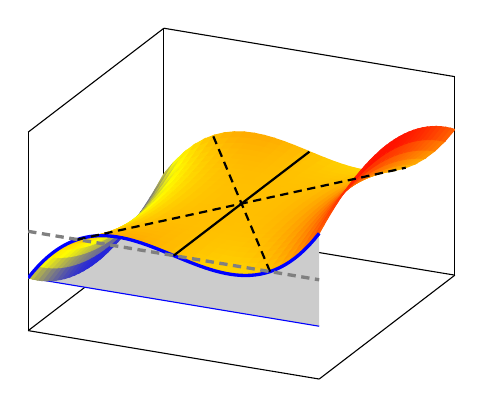
\begin{tikzpicture}
\begin{axis}[
%height=15cm,
%hide axis,
%axis lines=center,
%axis on top,
%axis line style={draw=none},
%tick style={draw=none},
xtick=\empty,
ytick=\empty,
ztick=\empty,
]
\newcommand{\xxx}{1.51}
\newcommand{\rrr}{-1}
\addplot3+[name path=A,blue,domain=-\xxx:\xxx,samples=60,samples y=0,mark=none] 
		({x},
		 {-1},
		 {20*(-\xxx)*(-\xxx-\rrr)*(-\xxx-1)});
\addplot3 [
surf,
shader=flat,
%faceted color=gray,
samples=30,
domain=-\xxx:\xxx,y domain=-1:1
] {20*x*(x+y)*(x+\rrr*y)};
\addplot3+[name path=B,blue,very thick,domain=-\xxx:\xxx,samples=60,samples y=0,mark=none] 
		({x},
		 {-1},
		 {20*x*(x-\rrr)*(x-1)});
\addplot3[gray!40] fill between[of=A and B];
\addplot3+[black,thick,domain=-1:1,samples=60,samples y=0,mark=none] 
		({0},
		 {x},
		 {0});
\addplot3+[black,thick,domain=-1:1,samples=60,samples y=0,mark=none] 
		({-x},
		 {x},
		 {0});
\addplot3+[black,thick,domain=-1:1,samples=60,samples y=0,mark=none] 
		({-\rrr*x},
		 {x},
		 {0});
\addplot3+[gray,very thick,domain=-\xxx:\xxx,samples=60,samples y=0,mark=none] 
		({x},
		 {-1},
		 {0});
\DrawDotThreeD{0}{-1}{0}
\DrawDotThreeD{1}{-1}{0}
\DrawDotThreeD{-1}{-1}{0}
\end{axis}
\end{tikzpicture}
\end{document}